\documentclass[12pt,titlepage]{article}
\usepackage[margin=1.25in]{geometry}
\usepackage{graphicx,amsmath,minted}

%% Variables definition
\newcommand{\vSubject}{Database}
\newcommand{\vSubtitle}{Normalisation}
\newcommand{\vName}{Dicha Zelianivan Arkana}
\newcommand{\vNIM}{2241720002}
\newcommand{\vClass}{1i}
\newcommand{\vDepartment}{Information Technology}
\newcommand{\vStudyProgram}{D4 Informatics Engineering}

%% [START] Tikz related stuff
\usepackage{tikz}
\usetikzlibrary{svg.path,calc,shapes.geometric,shapes.misc}
\tikzstyle{terminator} = [rectangle, draw, text centered, rounded corners = 1em, minimum height=2em]
\tikzstyle{preparation} = [chamfered rectangle, chamfered rectangle sep=0.75em, draw, text centered, minimum height = 2em]
\tikzstyle{process} = [rectangle, draw, text centered, minimum height=2em]
\tikzstyle{decision} = [diamond, aspect=2, draw, text centered, minimum height=2em]
\tikzstyle{data}=[trapezium, draw, text centered, trapezium left angle=60, trapezium right angle=120, minimum height=2em]
\tikzstyle{connector} = [line width=0.25mm,->]
%% [END] Tikz related stuff

%% [START] Fancy header related stuff
\usepackage{fancyhdr}
\pagestyle{fancy}
\setlength{\headheight}{15pt} % compensate fancyhdr style
\fancyhead{}
\fancyfoot{}
\fancyfoot[L]{\thepage}
\fancyfoot[R]{\textit{\vSubject - \vSubtitle}}
\renewcommand{\footrulewidth}{0.4pt}% default is 0pt, overline for footer
%% [END] Fancy header related stuff

%% [START] Custom tabular command related stuff
\usepackage{tabularx}
\newcommand{\details}[2]{
    #1 & #2  \\
}
%% [END] Custom tabular command related stuff

%% [START] Figure related stuff
\newcommand{\image}[3][1]{
    \begin{figure}[h]
        \centering
        \includegraphics[#1]{#2}
        \caption{#3}
        \label{#3}
    \end{figure}
}
%% [END] Figure related stuff

\begin{document}
\begin{titlepage}
    \centering
    \vfill
    {\bfseries\LARGE
        \vSubject\\
        \vskip0.25cm
        \vSubtitle
    }
    \vfill
    
\includegraphics[width=6cm]{images/polinema-logo.png}
    \vfill
    {
        \textbf{Name}\\
        \vName\\
        \vskip0.5cm
        \textbf{NIM}\\
        \vNIM\\
        \vskip0.5cm
        \textbf{Class}\\
        \vClass\\
        \vskip0.5cm
        \textbf{Department}\\
        \vDepartment\\
        \vskip0.5cm
        \textbf{Study Program}\\
        \vStudyProgram
    }
\end{titlepage}

\section{Hands-On}

\begin{figure}[h]
    \centering
    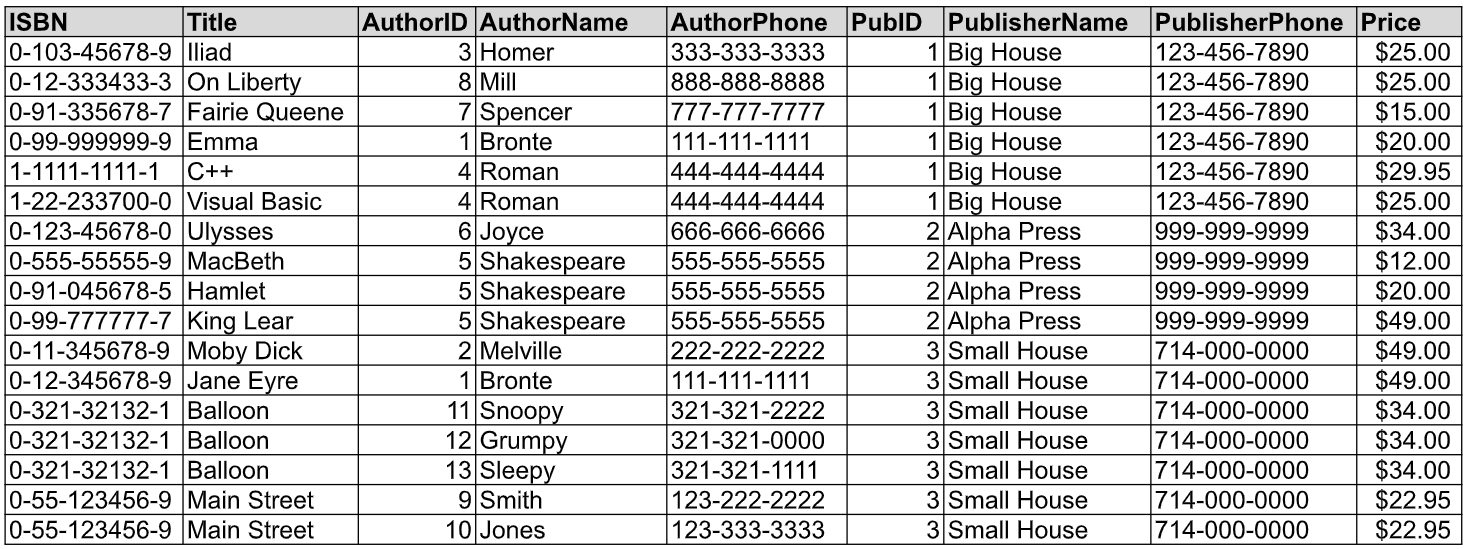
\includegraphics[width=\textwidth]{images/un-normalised.png}
    \caption{Un-normalised BOOKSHELF}
\end{figure}

\begin{enumerate}
    \item {
        Convert the table into normalised relation and give proper names for the tables

        \begin{figure}[h]
            \centering
            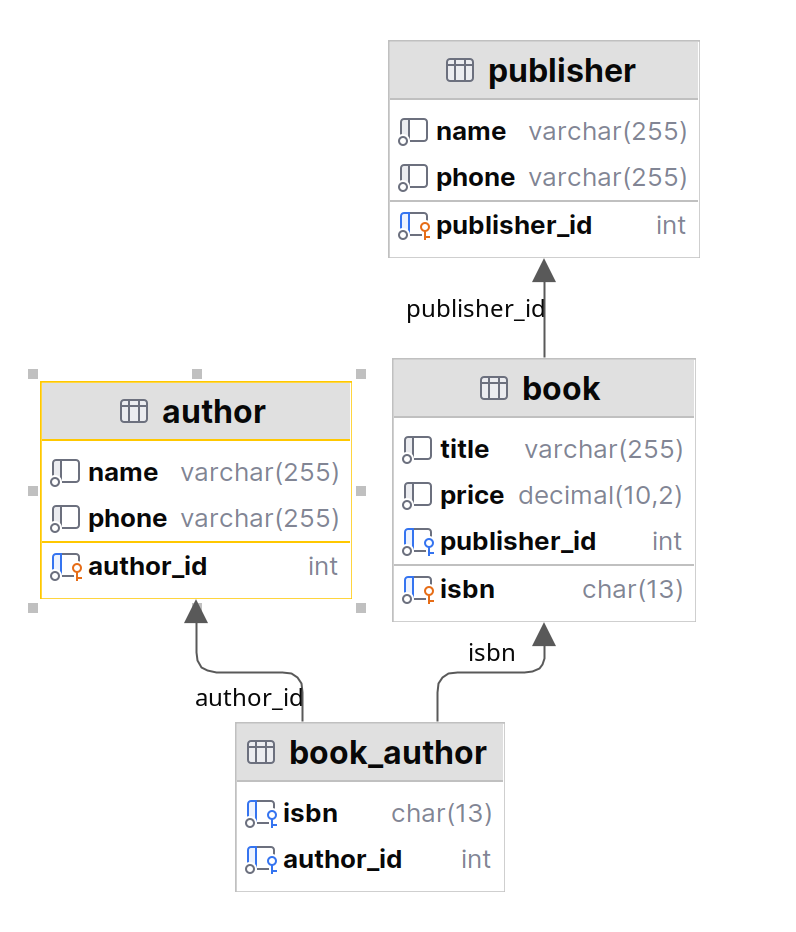
\includegraphics[width=.45\textwidth]{images/bookshelf-erd.png}
            \caption{Normalised BOOKSHELF}
        \end{figure}

        \begin{figure}[h]
            \centering
            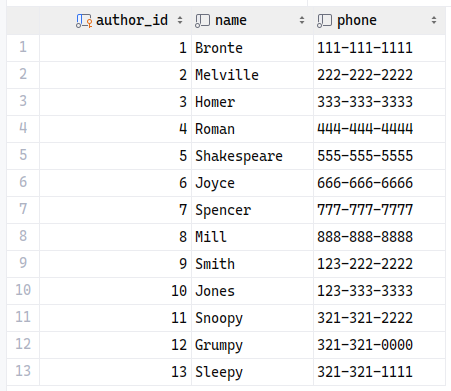
\includegraphics[width=.45\textwidth]{images/author-table.png}
            \caption{Author table}
        \end{figure}

        \begin{figure}[h]
            \centering
            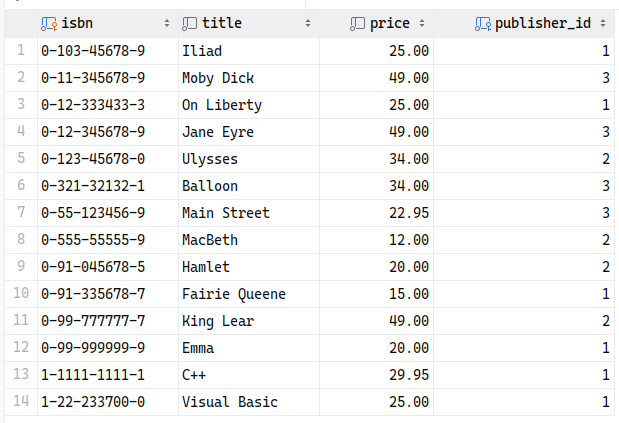
\includegraphics[width=.45\textwidth]{images/book-table.png}
            \caption{Book table}
        \end{figure}

        \pagebreak

        \begin{figure}[h]
            \centering
            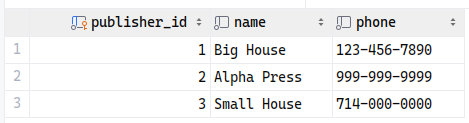
\includegraphics[width=.45\textwidth]{images/publisher-table.png}
            \caption{Publisher table}
        \end{figure}
        
        \pagebreak

        \begin{figure}[h]
            \centering
            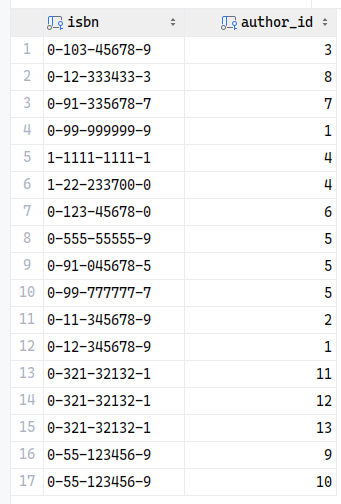
\includegraphics[width=.45\textwidth]{images/book-author-table.png}
            \caption{Book-Author table}
        \end{figure}
    }
    \pagebreak
    \item {
        Check if your new database can answer the following queries:

        \begin{enumerate}
            \item {
                Regenerate the original table as shown above using the \\
                normalised database

                \begin{minted}[autogobble,fontsize=\small]{sql}
                    CREATE TABLE book
                    (
                        isbn         CHAR(13)       NOT NULL PRIMARY KEY,
                        title        VARCHAR(255)   NOT NULL,
                        price        DECIMAL(10, 2) NOT NULL,
                        publisher_id INT            NOT NULL
                    );

                    CREATE TABLE author
                    (
                        author_id INT          NOT NULL PRIMARY KEY,
                        name      VARCHAR(255) NOT NULL,
                        phone     VARCHAR(255) NOT NULL
                    );

                    CREATE TABLE book_author
                    (
                        isbn      CHAR(13) NOT NULL,
                        author_id INT      NOT NULL
                    );

                    CREATE TABLE publisher
                    (
                        publisher_id INT          NOT NULL PRIMARY KEY,
                        name         VARCHAR(255) NOT NULL,
                        phone        VARCHAR(255) NOT NULL
                    );

                    ALTER TABLE book
                        ADD FOREIGN KEY (publisher_id) REFERENCES publisher (publisher_id);
                    ALTER TABLE book_author
                        ADD FOREIGN KEY (isbn) REFERENCES book (isbn);
                    ALTER TABLE book_author
                        ADD FOREIGN KEY (author_id) REFERENCES author (author_id);
                \end{minted}
            }
            \pagebreak
            \item {
                Display all books authored by Shakespeare

                \begin{minted}[autogobble,fontsize=\small]{sql}
                    SELECT
                        book.isbn as isbn, title, publisher.name as publisher_name, price
                    FROM
                        book_author
                    INNER JOIN book
                        ON book_author.isbn = book.isbn
                    INNER JOIN author
                        ON book_author.author_id = author.author_id
                    INNER JOIN publisher
                        ON book.publisher_id = publisher.publisher_id
                    WHERE author.name = 'Shakespeare';
                \end{minted}

                \begin{figure}[h]
                    \centering
                    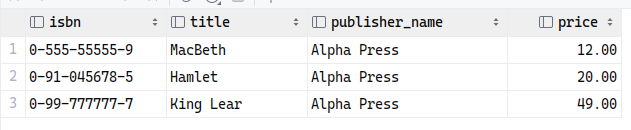
\includegraphics[width=.75\textwidth]{images/q1.png}
                    \caption{Query Result}
                \end{figure}
            }
            \pagebreak
            \item {
                Count the number of Books authored by each author. (AuthorID, AuthorName, NumberofBooks)

                \begin{minted}[autogobble,fontsize=\small]{sql}
                    SELECT
                        author.author_id as author_id,
                        author.name as author_name,
                        COUNT(author.name) as number_of_books
                    FROM book_author
                    INNER JOIN book
                        ON book_author.isbn = book.isbn
                    INNER JOIN author
                        ON book_author.author_id = author.author_id
                    GROUP BY author.author_id;
                \end{minted}

                \begin{figure}[h]
                    \centering
                    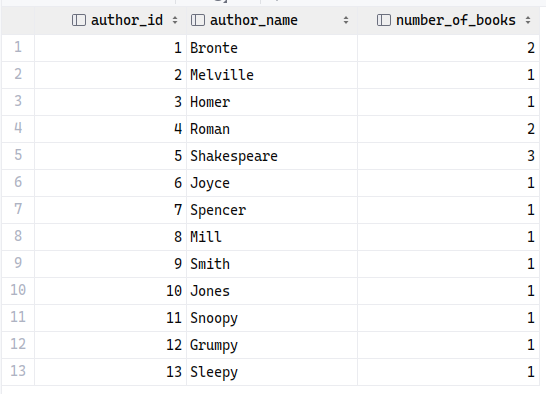
\includegraphics[width=.75\textwidth]{images/q2.png}
                    \caption{Query Result}
                \end{figure}
            }
            \pagebreak
            \item {
                What are the books authored by Shakespeare or Roman, displaying the ISBN, Title,
                Authorname, PublisherName, Price

                \begin{minted}[autogobble,fontsize=\small]{sql}
                    SELECT
                        book.isbn as isbn,
                        title,
                        author.name as author_name,
                        publisher.name as publisher_name,
                        price
                    FROM
                        book_author
                    INNER JOIN book
                        ON book_author.isbn = book.isbn
                    INNER JOIN author
                        ON book_author.author_id = author.author_id
                    INNER JOIN publisher
                        ON book.publisher_id = publisher.publisher_id
                    WHERE author.name = 'Shakespeare' or author.name = 'Roman';
                \end{minted}

                \begin{figure}[h]
                    \centering
                    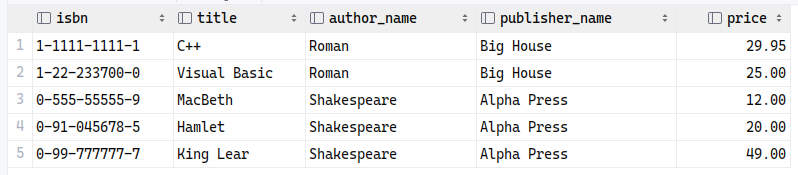
\includegraphics[width=.75\textwidth]{images/q3.png}
                    \caption{Query Result}
                \end{figure}
            }
            \pagebreak
            \item {
                Display the books (ISBN, Title, AuthorID, AuthorName) publised by Small

                \begin{minted}[autogobble,fontsize=\small]{sql}
                    SELECT
                        book.isbn as isbn,
                        title,
                        author.author_id as author_id,
                        author.name as author_name
                    FROM
                        book_author
                    INNER JOIN book
                    ON book_author.isbn = book.isbn
                    INNER JOIN author
                    ON book_author.author_id = author.author_id
                    INNER JOIN publisher
                            ON book.publisher_id = publisher.publisher_id
                    WHERE publisher.name = 'Small House';
                \end{minted}

                \begin{figure}[h]
                    \centering
                    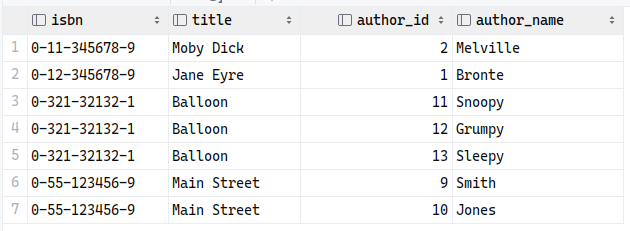
\includegraphics[width=.75\textwidth]{images/q4.png}
                    \caption{Query Result}
                \end{figure}
            }
            \pagebreak
            \item {
                What is the total price of the books published by each publisher. (PubID, PublisherName, TotalPrice)

                \begin{minted}[autogobble,fontsize=\small]{sql}
                    SELECT
                        publisher.publisher_id as publisher_id,
                        publisher.name as publisher_name,
                        SUM(book.price) as book_price
                    FROM
                        book
                    INNER JOIN publisher
                            ON book.publisher_id = publisher.publisher_id
                    GROUP BY publisher.publisher_id;
                \end{minted}

                \begin{figure}[h]
                    \centering
                    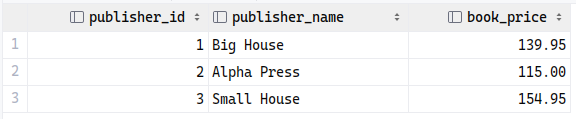
\includegraphics[width=.75\textwidth]{images/q5.png}
                    \caption{Query Result}
                \end{figure}
            }
            \item {
                How many books were published by each publisher? (PubID, PublisherName, NumberofBooks)

                \begin{minted}[autogobble,fontsize=\small]{sql}
                    SELECT
                        publisher.publisher_id as publisher_id,
                        publisher.name as publisher_name,
                        COUNT(publisher.publisher_id) as number_of_books
                    FROM
                        book
                    INNER JOIN publisher
                       ON book.publisher_id = publisher.publisher_id
                    GROUP BY publisher.publisher_id;
                \end{minted}

                \begin{figure}[h]
                    \centering
                    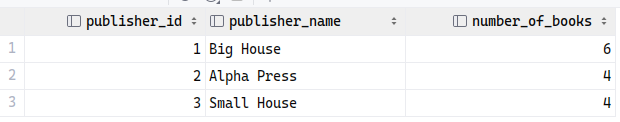
\includegraphics[width=.75\textwidth]{images/q6.png}
                    \caption{Query Result}
                \end{figure}
            }
        \end{enumerate}
    }
\end{enumerate}



\end{document}

